\section{Inteligencia de negocio}

La programación por restricciones \cite{Francesca} es una herramienta poderosa para solucionar problemas combinatorios. La programación por restricciones utiliza técnicas de diferentes áreas, por ejemplo de inteligencia artificial, ciencias de la computación y lenguajes de programación. La programación por restricciones es actualmente aplicada para problemas de muchos dominios, como son la programación de tareas, planeación, búsqueda de caminos o rutas para llegar a un punto, redes de comunicación y bioinformática. 
\\ \\
La idea básica en programación por restricciones es que el usuario escriba las restricciones y un solucionador de propósito general halle una solución. Las Restricciones son relaciones y un problema de satisfacción de restricciones (CSP) contiene las relaciones entre las variables de decisión. Los modelos de restricciones, son representados en términos de variables de decisión y restricciones, a partir de ellos, se debe encontrar una asignación de todas las variables que satisfaga las restricciones. Los solucionadores para programación por restricciones buscan sistemáticamente la solución en un espacio de búsqueda, con algoritmos de \textit{Backtracking} o \textit{Branch and Bound}. El método de búsqueda sistemático busca la interpolación, se conoce como la propagación de la información contenida en una restricciones a otras restricciones, lo que reduce el espacio de búsqueda de valores para un conjunto de variables.

\subsection{Problemas de satisfacci\'on de restricciones.}

Un problema de satisfacción de restricciones \cite{Krzysztof} se define así:

\begin{itemize}
\item Variables $y_{1},y_{2},...,y_{n}$
\item Dominios  $D_{1},D_{2},...,D_{n}$
\item Restricciones  $C: y_{1} \in D_{1},y_{2} \in D_{2},...,y_{n} \in D_{n}$
\end{itemize}

Una solución es:

$$(d_{1},d_{2},...,d_{n}) \in D_{1}*D_{2}*...*D_{n}$$

Donde se cumplen las restricciones C, es decir:

$$(d_{1},d_{2},...,d_{n}) \in C $$

\subsection{Satisfacci\'on de restricciones}

La satisfacción de restricciones \cite{Francesca}, es básicamente encontrar un valor para cada una de las variables del problema. Las restricciones podan los posibles valores de las variables; para conseguir un solución al problema se utilizan estrategias de búsqueda.
\\ \\
La estrategia de búsqueda fundamental es el \textit{Backtracking} o vuelta hacia atrás, que consiste en realizar un recorrido en un árbol o grafo dirigido que no contiene ciclos. El objetivo es recorrer la estructura hasta encontrar soluciones, lo que se consigue obteniendo soluciones parciales a medida que progresa el recorrido; las soluciones parciales limitan las regiones donde se puede encontrar una solución completa. La búsqueda tiene éxito, si se puede encontrar una solución completa, el algoritmo puede detenerse o buscar soluciones alternativas. Si no encuentra una solución en un recorrido por una parte de la estructura del grafo dirigido o árbol, vuelve hacia atrás de forma similar a la de un recorrido por profundidad, eliminando los elementos que se hubieren añadido en cada fase.

\subsection{Propagaci\'on de restricciones}

La propagación de restricciones \cite{Krzysztof} es un concepto general, que consiste en encontrar relaciones entre restricciones usando algoritmos de filtrado, interferencia de restricciones, reglas de interacción e interacciones caóticas. 
\\ \\
La propagación de restricciones embebe cualquier razonamiento que consista en prohibir cualquier valor o combinación de valores para algunas variables de un problema a causa de que un subgrupo de restricciones no pueden ser satisfechas.

\subsubsection{Arco consistencia:} 

La arco consistencia es la más conocida de todas las formas de propagación de restricciones. Para que un CSP sea arco consistente se requiere que:
\\ \\
Para un conjunto de variables $X$ e $Y$, se requiere que $ \forall X \in dom(X)$ $\exists Y \in dom(Y)$ tal que $r(X,Y)$ esta satisfecha y sea recíproca, es decir para todo $\forall Y \in dom(Y) \exists x \in dom(X) $ tal que $r(X,Y)$ esta satisfecha.

\subsection{Estrategias de búsqueda}

Una estrategia de búsqueda \cite{Krzysztof} consiste en un árbol de búsqueda y un algoritmo de búsqueda el cual explorar el árbol nodo a nodo para encontrar soluciones a un problema de programación por restricciones específico. Existen dos grandes estrategias de búsqueda la \textit{Branch and Bound} y el \textit{Backtrack}.

\subsubsection{Árbol de búsqueda}

Un árbol de búsqueda está representado de la siguiente manera
\begin{figure}[H]
	\centering
	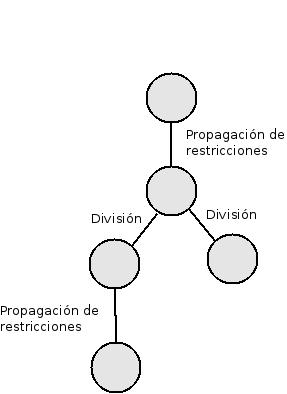
\includegraphics[width=5cm]{Capitulo2MarcoTeorico/Imagenes/Restri.jpeg}
	\caption{Estructura de un árbol de búsqueda}
	\label{fig:busqueda}	
\end{figure}

En la figura \ref{fig:busqueda} las operaciones de propagación de restricciones indican que al aplicar una restricción a un dominio finito $D$ éste se conserva o se reduce para obtener un dominio $D^{'}$. El momento en que se realizan las operaciones de división, es cuando no se puede propagar más las restricciones y el resultado es la división del dominio $D$ en $n$ dominios $D_{1}, ... ,D_{n}$


\subsubsection{Algoritmo Backtrack}

Este algoritmo construye una solución iniciando con una instancia vacía y sucesivamente intenta extender hasta obtener una instancia consistente definida por las siguientes variables. Si el procedimiento obtiene que la variable final obtiene una instanciación se encuentra una solución.
\\\\
Bajo esta premisa se han elaborado muchas estrategias de búsqueda como son \textit{Backtrack-free search with constraint propagation} y \textit{Backtrack-free Search}.
\\\\
Estas no son objeto de estudio, ya que en el proyecto se utiliza la estrategia \textit{Branch and Bound} programada en \textit{Mozart OZ}.

\subsubsection{Branch and Bound}

En este algoritmo existen dos grandes procedimientos:

\begin{itemize}
	\item \textbf{Ramificación:} La expansión del árbol de búsqueda está condicionado por la búsqueda de la mejor solución, con esto se exploran todos los nodos de una rama hasta explorar en un nuevo nivel.
	\item \textbf{Poda:} El objetivo es eliminar aquellos nodos que no lleven a soluciones buenas, con esto se busca evitar expandirlos ya que sus hijos tampoco serán buenas soluciones.
\end{itemize}

Esta es una de las mejores estrategias para realizar búsquedas ya que evita expandir todo el árbol, para obtener ganancias en velocidad de procesamiento y uso de memoria.

\subsubsection{Motores de búsqueda}

Son algoritmos que permiten filtrar las soluciones encontradas por un algoritmo de búsqueda, por ejemplo seleccionar las soluciones que mejoran un costo determinado. Con éstos motores se busca encontrar la mejor solución a un problema de acuerdo a criterios de costo propios del problema.

\subsubsection{Recomputación}

Durante el proceso de expansión de un árbol de búsqueda\cite{MultiOZ} se almacena en memoria la información de cada nodo expandido; con esto se busca evitar que se calcule de nuevo un nodo si el algoritmo de búsqueda va hacia atrás. Un nivel de recomputación $n$ indica que se almacenan los nodos que quedan a una distancia $n$ de un nodo que se encuentra guardado. La recomputación es útil para árboles de búsqueda muy grandes donde se requiere una gran cantidad de memoria para su almacenamiento pero tiene un costo adicional de procesamiento al tener que calcular de nuevo los nodos no almacenados en memoria. 

\subsection{Estrategias de distribución}

Una estrategia de distribución\cite{RestriCurso} define la forma y el contenido del árbol de búsqueda, cuántas alternativas existen en un nodo y qué restricción se agrega por cada alternativa. Las estrategias de distribución se utilizan para mejorar el rendimiento de los algoritmos de búsqueda, ya que una definición apropiada de un árbol de búsqueda permite guiar la exploración para encontrar más rápido la solución óptima.



